\section{Introduction}
The powerful semantic capabilities of modern  language models (LLMs) create exciting opportunities for building AI-based analytics systems that reason over vast knowledge corpora. Many applications require complex reasoning over large amounts of data, including both unstructured and structured data. For example a researcher reviewing recent ArXiv~\cite{arxivorg} pre\-prints may want to quickly obtain a summary of relevant papers from the past week, or find the papers that report the best performance for a particular task and dataset. Similarly, a medical professional may automatically extract biomedical characteristics and candidate diagnoses from many patient reports~\cite{doosterlinck_biodex_2023}. Likewise, organizations wish to automatically digest lengthy transcripts from internal meeting transcripts and chat histories to validate hypotheses about their business~\cite{discovery}.

Each of these tasks require a form of \emph{bulk semantic processing}, where the analytics system must process large amounts of data and apply semantic-based analysis 
across a whole dataset. Supporting the full generality of these applications with efficient and easy-to-use analytics systems would have a transformative impact, similar to what RDBMSes had for tabular data. This prospect, however, raises two challenging questions: first, \emph{how should developers express semantic queries}, and secondly, \emph{how should we design the underlying analytics system to achieve high efficiency and accuracy}.

\begin{figure}[!t]
  \centering
  % \vspace{-.4cm}
  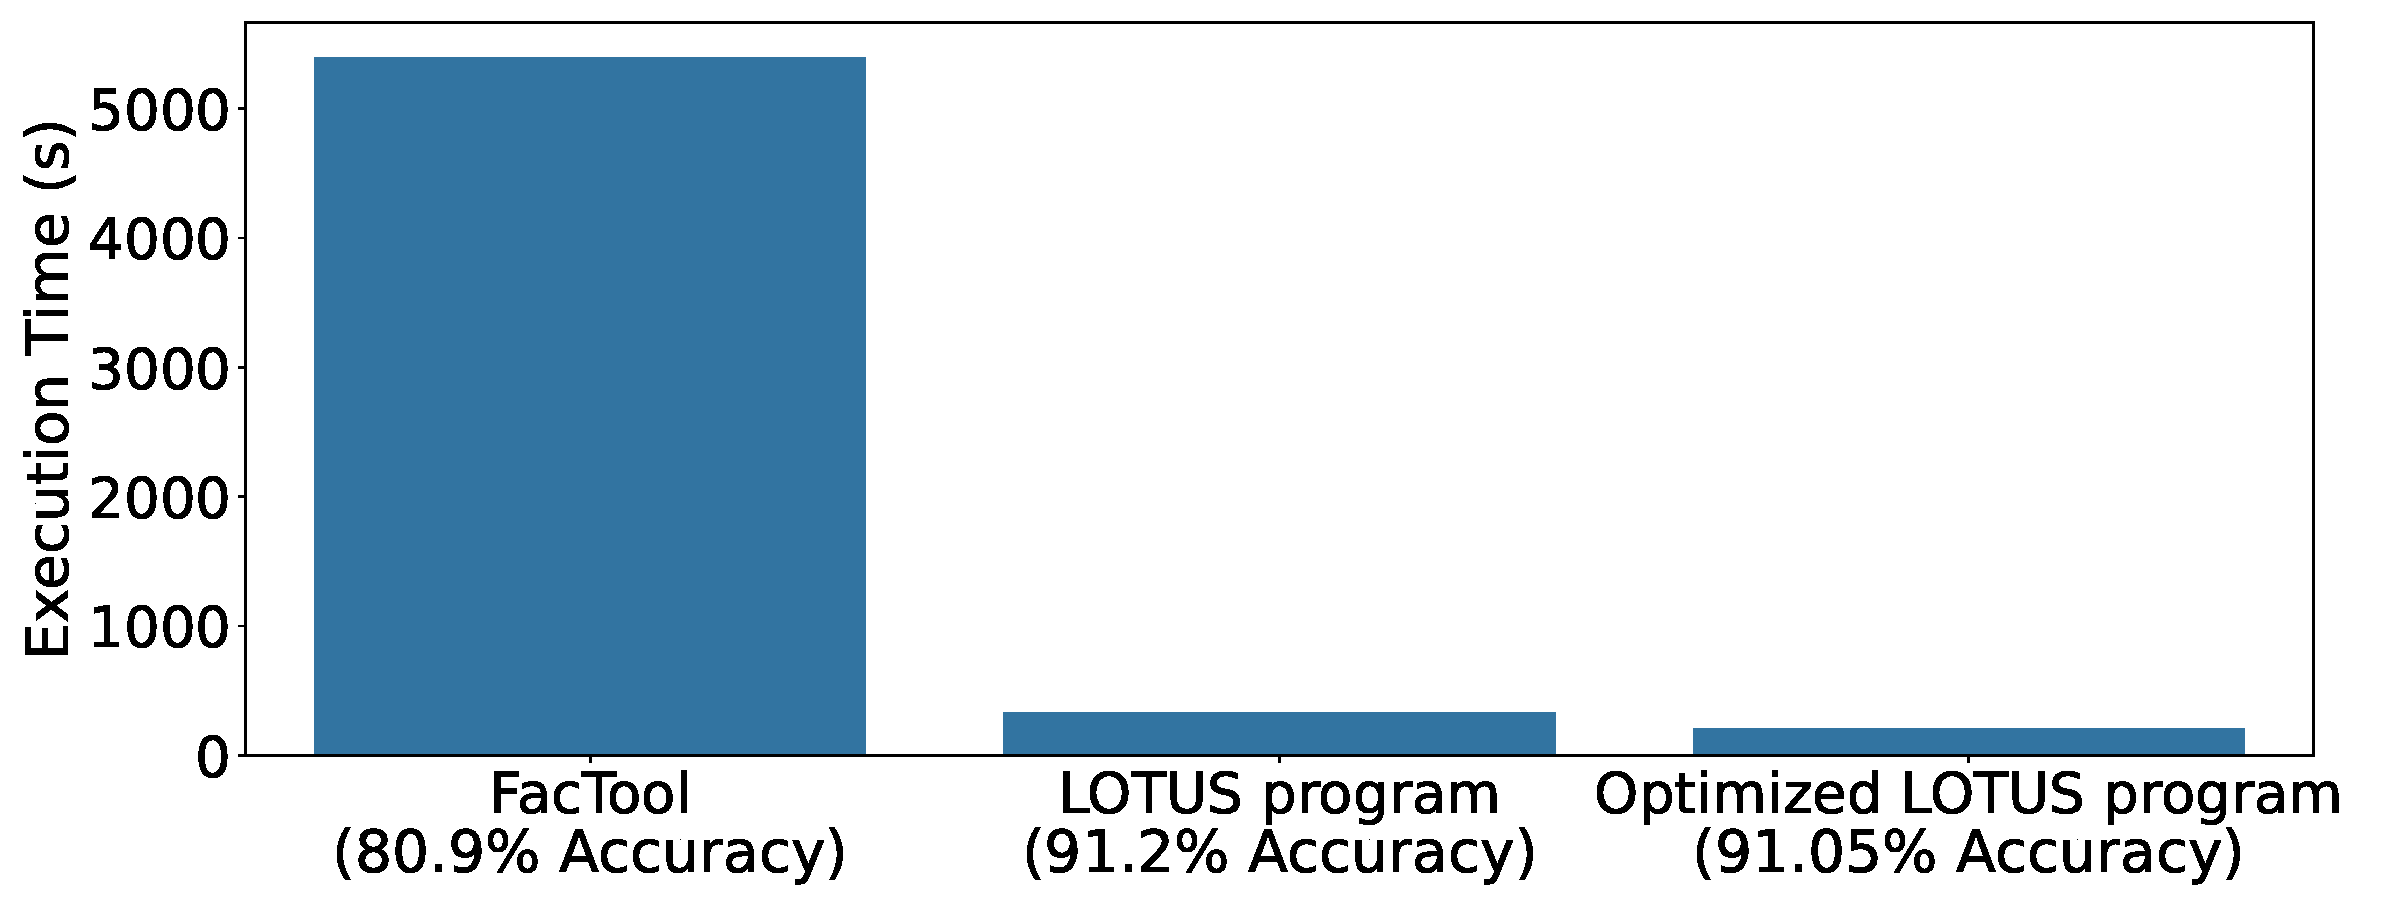
\includegraphics[width=\linewidth]{figures/factchecking.pdf}
  \vspace{-.6cm}
  \caption{\small Execution time (y-axis) and accuracy, shown in parentheses, for 3 fact-checking implementations: (i) FacTool~\cite{chern_factool_2023}, a recent state-of-the-art research work, (ii) a short, un-optimized \sys program, and (iii) the same \sys program optimized with accuracy guarantees. Section~\ref{sec:eval} provides our full methodology.}
  \label{fig:factchecking_plot}
   \vspace{-.3cm}
\end{figure}


Unfortunately, existing systems are insufficient for bulk semantic processing, either limiting their expressiveness to row-wise LLM execution models or focusing on empirical optimizations without any formalism or accuracy guarantees, leading to unexpected behaviors and frequent failures. 
First, several systems provide logically row-wise LLM operators, either in the form of a general-purpose AI user-defined functions (UDF)~\cite{motherduck_introducing_nodate, williamdassafmsft_intelligent_2024, noauthor_snow_nodate, vertexai, databricks, noauthor_large_nodate, liu_optimizing_2024} or specialized row-wise operators~\cite{liu_suql_2024, liu_declarative_2024, lin_towards_2024} for specific applications, such as conversational chat, data cleaning and extract-transform-load (ETL) tasks. These programming models fail to support a range of LLM-based transformations \emph{across} rows, such as ranking, grouping or joining records. Alternatively, more recent LLM-based analytics systems, such as DocETL~\cite{shankar_docetl_2024} and UQE~\cite{dai_uqe_2024}, empirically optimize LLM-based operations with no accuracy guarantees, lacking any formalism to define correct behavior, which hinders their robustness and usability, as we show in Section~\ref{sec:eval}. These obstacles highlight a core challenge of integrating semantic-based processing within reliable query systems due to the inherent ambiguity of natural language instructions and LLM outputs.


% \begin{figure}[!t]
%     \centering
%     \begin{lstlisting}[language=Python]
% def get_paper_digest(papers_df, projects_df):
%   return papers_df\
%     .sem_join(projects_df, "the paper {abstract:left} is highly relevant to my {research_areas:right}")\
%     .sem_map("What is the key insight of the {abstract} and how does it relate to my {research_areas}", name="insights")\
%     .sem_agg("Write a digest summarizing the research {insights}")
% \end{lstlisting}
%     \vspace{-.4cm}
%     \caption{\small Example \sys program using semantic operators to return a summary of relevant papers. The user function, takes two strings, describing research interests and a research baseline. The program searches over papers, then filters based on whether each paper outperforms the baseline, and finally constructs a summary.}
%     \label{fig:example_code}
%     \vspace{-.5cm}
% \end{figure}

\begin{figure*}[th]
  \centering
  % \vspace{-.4cm}
  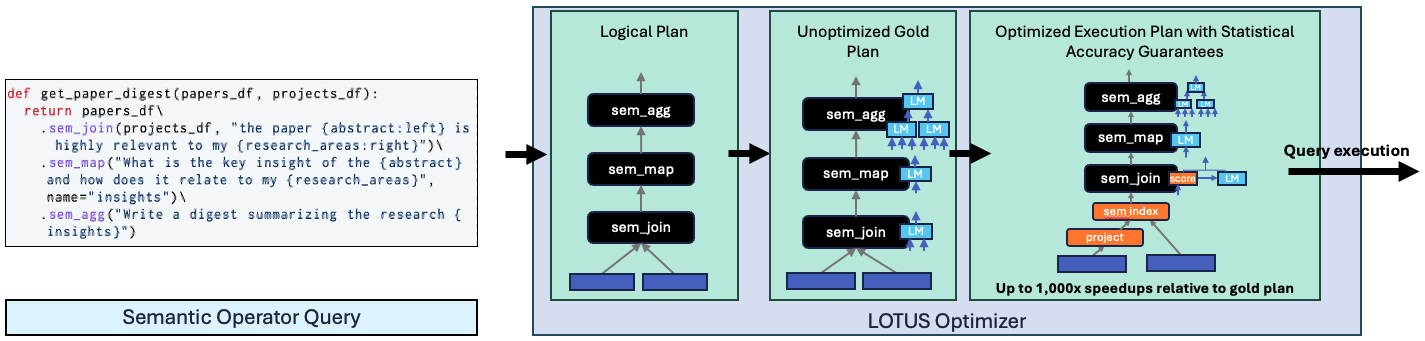
\includegraphics[width=\linewidth]{figures/summary_figure.png}
  % \vspace{-.6cm}
  \caption{\small An example semantic operator query is shown on the left. The user function takes two two datasets and uses a series of semantic operators to to create a summary of relevant research papers from papers\_df based on the user's research areas from projects\_df. Given a user's query, LOTUS defines a logical plan, which it then converts to an un-optimized gold plan, that specifies how to orchestrate the LM over the data. LOTUS then generates an optimized execution plan with statistical accuracy guarantees relative to the gold plan. These optimized plans empirically demonstrate up to $1,000\times$ speedups. Finally, LOTUS executes the optimized plan and returns the results to the user.}
    \label{fig:example_code}
   % \vspace{-.3cm}
\end{figure*}


Towards robust, declarative query systems for bulk semantic processing, we propose the \emph{semantic operator model}, which extends the relational model with AI-based operations. Semantic operators provide the first formalism for general-purpose and multi-row, AI-based transformation, including semantic filters, joins, top-k rankings, aggregations, and projections. Each operator takes a concise natural language signature, given by the programmer, and its behavior is fully specified by a tractable, high-quality "gold" algorithm, which indicates how to orchestrate the underlying AI model over the data. 
Our optimization approach then exploits the rich design space of semantic operator execution plans to reduce cost, while providing \emph{statistical accuracy guarantees} with respect to the gold algorithm (i.e., guarantees that the output of the optimized operator will be similar to that of the gold algorithm). 
We propose several novel optimizations for the semantic filter, join, top-k and group-by operators.
Our methods include approximation algorithms, building on statistical techniques used in prior works~\cite{kang_accelerating_2021, kang_approximate_2020} with novel and efficient proxy scorers using small LLMs or semantic embeddings. 
We implement semantic operators in \sys 
(\textbf{L}LMs \textbf{O}ver \textbf{T}ables of \textbf{U}nstructured and \textbf{S}tructured data), an open source system that exposes these operators through a simple DataFrame-based programming interface.  



\begin{footnotesize}
    
\begin{table*}[!t]
\newcolumntype{C}[1]{>{\raggedright\arraybackslash}p{#1}}
\renewcommand{\arraystretch}{1.4} % Adjust the value to increase/decrease row spacing
\centering
\caption{\small Summary of Key Semantic Operators. $T$ denotes a relation, $X$ and $Y$ denote arbitrary tuple types. $l$ denotes a parameterized natural language expression (``langex`` for short). Each operator may permit additional optional parameters, including accuracy targets.}
\vspace{-.3cm}
\begin{tabular}{C{4.1cm}C{5cm}C{4.1cm}C{4.2cm}}
% \begin{tabular}{ccccc}
% \hline
\toprule
\textbf{Operator} & \textbf{Description}  & \textbf{Definition} &  \textbf{Gold Algorithm}\\
% \hline
\midrule
$\mathit{sem\_filter}(l\textit{: } X \rightarrow \mathit{Bool})$ 
& Returns the tuples that pass the langex predicate. 
% & $l: X\rightarrow Bool$
& $\{t_i \in T | l_M(t_i) = 1\}$
& Compute $M(t_i, l) \forall t_i\in T$ \\
% \hline


$\mathit{sem\_join}(t\textit{: } T \comma l\textit{: } (X, Y) \rightarrow \mathit{Bool})$ 
& Joins a table against a second table $t$ by keeping all tuple pairs that pass the langex predicate. 
% & $l: X\rightarrow Bool$
& $\{(t_i, t_j) | l_M(t_i, t_j) = 1, t_i \in T_1, t_j\in T_2 \}$
& Compute $M(t_i, t_j, l) \forall t_i\in T_1, t_j\in T_2$ \\
% \hline


$\mathit{sem\_agg}(l\textit{: } T[X] \rightarrow \mathit{X})$ 
& Aggregates input tuples according to the langex reducer function.
% & $l: Set[X]\rightarrow X$
& $l_M(t_1, ..., t_n) \forall t_1, .., t_n \in T$
& Perform a reduce algorithm, recursively computing $a_{i+1, j} = M(a_{i, f(j)}, ..., a_{i, f(j)+n'}, l)$, $a_{0, j} = M(t_{f(j)}, ..., t_{f(j)+n'}, l)$ 
\\
% \hline


$\mathit{sem\_topk}(l\textit{: } T[X] \rightarrow Seq[X]\comma k\textit{: }int)$ & Returns an ordered list of the $k$ best tuples according to the langex ranking criteria.
% & $l: T[X]\rightarrow Seq[X]$
& $\langle t_1, ..., t_k\rangle \textit{ st } \forall (t_i, t_j), i < j \implies  l_M(t_i, t_j) = \langle t_i, t_j\rangle $
& Perform top-k sorting algorithm using pairwise comparisons, $M(t_i, t_j, l)$\\
% \hline


$\mathit{sem\_group\_by}(l\textit{: } X \rightarrow Y\comma C\textit{: } int)$ & Groups the tuples into $C$ categories based on the langex grouping criteria. 
% & $l: X \rightarrow Y$
& $\underset{\{\mu_1, ...\mu_C\}, \mu_i \in V^\mathbb{N}}\argmax\textit{\space} \underset{t_i\in T}\sum \underset{j\in 1\ldots C}\max l_{M}(t_i, \mu_j)$
& Obtain centers $\mu_1, ...\mu_C$ with a clustering algorithm, and perform pointwise assignments $M(t_i, \mu_1, ..., \mu_C) \forall t_i\in T$\\

$\mathit{sem\_map}(l\textit{: } X \rightarrow Y)$ & Performs the projection specified by the langex. 
% & $l: X\rightarrow Y$
& $\{l_M(t_i), \forall t_i \in T\}$
& Compute $M(t_i, l) \forall t_i\in T$\\

% \hline
\bottomrule
\label{tab:operators}

\end{tabular}
\vspace{-1.0cm}

\end{table*}

\end{footnotesize}





Figure \ref{fig:factchecking_plot} illustrates the power of \sys' declarative programming model and optimized query engine. For a fact-checking task on the FEVER dataset \cite{thorne_fever_2018},  we  write an intuitive \sys program to re-implement a recent state-of-the-art fact-checking pipeline, FacTool~\cite{chern_factool_2023}, which was originally implemented in over 750 lines of code. Our un-optimized \sys program composes $3$ semantic operators (filters, maps and joins)  and achieves  $12.7\%$ higher accuracy on this task. \sys also provides query efficiency by default, yielding $28\times$ lower execution time than the original FacTool implementation.
Furthermore, the optimized \sys program, configured with $0.9$ accuracy targets and a $0.2$  allowed error probability,  runs $1.7\times$ faster and obtains $99.8\%$ accuracy compared to the un-optimized \sys program.

We systematically evaluate \sys on four real bulk-semantic processing applications:  fact-checking, biomedical multi-label classification, search, and topic analysis. 
These include applications expressible and studied by recent LLM-based analytics systems~\cite{shankar_docetl_2024, dai_uqe_2024}, where we compare against those systems, as well as others, where we compare against hand-designed pipelines from the AI literature. 
% \liana{this needs to be about comparison to all baselines}
We demonstrate that the semantic operator model is effective, capturing state-of-the-art AI pipelines in a few operator calls that reliably match or exceed quality of recent LLM-based analytics systems by up to $100\%$, while offering accuracy guarantees and running up to $3.6\times$ faster than the best-quality baselines. 
% reproducing state-of-the-art query results in short, intuitive programs for each applications. 
Furthermore, our gold algorithms provide high-quality results, and our optimizations speed up query execution by up to $1,000\times$ with respect to them.
Specifically, our \sys program re-implements FacTool's recent state-of-the-art fact-checking pipeline~\cite{chern_factool_2023}, as shown in Figure \ref{fig:factchecking_plot}, and achieves $12.5\%$ higher accuracy  with $28\times$  lower execution time on the FEVER dataset ~\cite{thorne_fever_2018}, outperforming alternative LLM-powered analytics systems on both accuracy and efficiency. In the extreme multi-label classification task on the BioDEX dataset~\cite{doosterlinck_biodex_2023}, \sys reproduces state-of-the art result quality~\cite{doosterlinck_-context_2024} and the LLM-powered analytics baselines, while providing  accuracy guarantees and $1,000\times$ speedups with respect to our gold algorithm. In the search and ranking application, \sys allows a simple composition of operators to achieve $3 -  100\%$ higher nDCG@10 than the next best performing baselines, while also providing query efficiency, with $1.67 - 10\times$ lower execution time than alternative high-quality algorithms. In the topic analysis task, \sys efficiently processes hundreds of ArXiv papers to discover a taxonomy of key topics in dozens of seconds, while once again providing configurable speedups with statistical accuracy guarantees.

Overall, our main contributions are the following:
\begin{itemize}
    \item We propose semantic operators, the first formalized programming model for general-purpose AI-based transformations with natural language specifications. 
    \item We define an optimization framework for semantic operators with statistical accuracy guarantees, and novel optimizations for several operators, including semantic filters, joins, top-k and group-by, yielding up to $1,000\times$ speedups.
    \item  We extensively evaluate the expressiveness of the semantic operator model, the quality of our gold algorithms, and the benefit of our optimizations, including comparisons to DocETL, UQE, and AI UDFs. 
\end{itemize}


